\centering
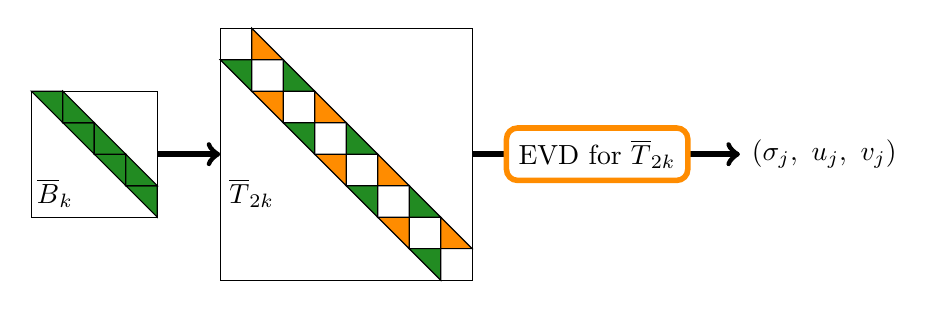
\begin{tikzpicture}[scale=.4]
  \pgfmathsetmacro{\ix}{1}
  \begin{scope}
    \draw[fill=white] (0,-2) rectangle +(4,4);
    \foreach \x in { 0,...,3 }
    \draw[fill=ForestGreen] (\x*\ix+\ix,2-\ix-\x*\ix) -- (\x*\ix+\ix,2-\ix-\x*\ix+\ix) -- (\x*\ix,2-\ix-\x*\ix+\ix) -- cycle;
    \foreach \x in { 1,...,3 }
    \draw[fill=ForestGreen] (\x*\ix+\ix,2-\x*\ix) -- (\x*\ix,2-\x*\ix) -- (\x*\ix,2-\x*\ix+\ix) -- cycle;
    \draw (0.75,-1.25) node{$\overline{B}_k$};
  \end{scope}

  \begin{scope}[shift={(0:4)}]
    \draw [->,thick,line width=2pt] (0,0) -- (2,0);
  \end{scope}

  \begin{scope}[shift={(0:6)}]
    \draw[fill=white] (0,-4) rectangle +(8,8);
    \foreach \x in { 0,...,3 }
    \draw[fill=ForestGreen] (2*\x*\ix+\ix,2-2*\x*\ix) -- (2*\x*\ix+\ix,2-2*\x*\ix+\ix) -- (2*\x*\ix,2-2*\x*\ix+\ix) -- cycle;
    \foreach \x in { 0,...,2 }
    \draw[fill=DarkOrange] (2*\x*\ix+2*\ix,2-2*\x*\ix-\ix) -- (2*\x*\ix+2*\ix,2-2*\x*\ix) -- (2*\x*\ix+\ix,2-2*\x*\ix) -- cycle;
    \foreach \x in { 0,...,3 }
    \draw[fill=DarkOrange] (2*\x*\ix+2*\ix,3-2*\x*\ix) -- (2*\x*\ix+\ix,3-2*\x*\ix) -- (2*\x*\ix+\ix,4-2*\x*\ix) -- cycle;
    \foreach \x in { 1,...,3 }
    \draw[fill=ForestGreen] (2*\x*\ix+\ix,4-2*\x*\ix) -- (2*\x*\ix,4-2*\x*\ix) -- (2*\x*\ix,4-2*\x*\ix+\ix) -- cycle;
    \draw (1,-1.25) node{$\overline{T}_{2k}$};
  \end{scope}

  \begin{scope}[shift={(0:14)}]
    \draw [->,thick,line width=2pt] (0,0) --
    (1,0) node[right,align=center, text width=2cm,rounded corners,draw=DarkOrange,fill=white,inner sep=1ex]{EVD for $\overline{T}_{2k}$} --
    (8.5,0) node[right,align=center]{$\left(\sigma_j,\ \bm{u}_j,\ \bm{v}_j\right)$};
  \end{scope}
\end{tikzpicture}
